\documentclass[letterpaper, 10 pt, conference]{ieeeconf}  % Comment this line out if you need a4paper
\usepackage{epsfig}
\usepackage{graphicx}
\usepackage{color}
\usepackage[frenchb]{babel}
\usepackage{subfigure}
\usepackage{amsmath}
\usepackage{amssymb}
\usepackage{enumerate}

% Pour pouvoir utiliser les accents directement dans LaTeX, sans utiliser les commandes \'
%\usepackage[latin1]{inputenc} % entree 8 bits iso-latin1
\usepackage[T1]{fontenc}      % encodage 8 bits des fontes utilisees
\usepackage[utf8]{inputenc} % entree 8 bits utf8, fonctionne avec MikTeX sur Windows.


\overrideIEEEmargins                                      % Needed to meet printer requirements.

% See the \addtolength command later in the file to balance the column lengths
% on the last page of the document



\begin{document}
\selectlanguage{frenchb} 
\title{\LARGE \bf  Format du rapport GLO-7021}


\author{Jean Tremblay et John Smith}


\maketitle
\thispagestyle{empty}
\pagestyle{empty}


%%%%%%%%%%%%%%%%%%%%%%%%%%%%%%%%%%%%%%%%%%%%%%%%%%%%%%%%%%%%%%%%%%%%%%%%%%%%%%%%
\begin{abstract}

Résumé de l'article en un paragraphe. Doit comprendre a) Motivation b) Problématique c) Approche d) Résutlats e) Conclusion. Inspirez-vous de http://www.ece.cmu.edu/\tild koopman/essays/abstract.html .

\end{abstract}


%%%%%%%%%%%%%%%%%%%%%%%%%%%%%%%%%%%%%%%%%%%%%%%%%%%%%%%%%%%%%%%%%%%%%%%%%%%%%%%%
\section{Introduction}

blah blah blah.

\section{Description du projet et de la problématique, en lien avec la littérature}

\begin{equation}
E=mc^2
\label{Einstein}
\end{equation}

Je veux résoudre le problème de relativité décrit à l'équation~\ref{Einstein}! Et j'utilise~\cite{c1} comme article! La distance est de $d=3~m$.

\section{Approche proposée}
Voici une liste :
\begin{itemize}
\item Item 1;
\item Item 2.
\end{itemize}

\section{Protocole d'expérimentation}

\section{Résultats}

\subsection{Equations}

\subsection{Figures and Tables}


\begin{table}[h]
\caption{An Example of a Table}
\label{table_example}
\begin{center}
\begin{tabular}{|c||c|}
\hline
One & Two\\
\hline
Three & Four\\
\hline
\end{tabular}
\end{center}
\end{table}

\begin{figure}[thpb]
      \centering
      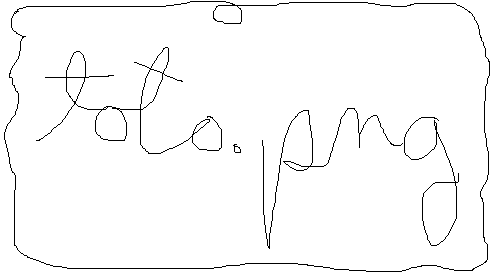
\includegraphics[width=0.47\textwidth]{toto.png}
      \caption{Dans matlab, vous pouvez produire des .png ou des .eps pour les figures. Voir la commande "print -dpng" ou "print -deps". Généralement, .eps donne de plus beaux rendus.}
      \label{MaFigure}
\end{figure}
   

Je référence la figure avec \ref{MaFigure}.

% Pour une figure double colonne
\begin{figure*}[thpb]
      \centering
      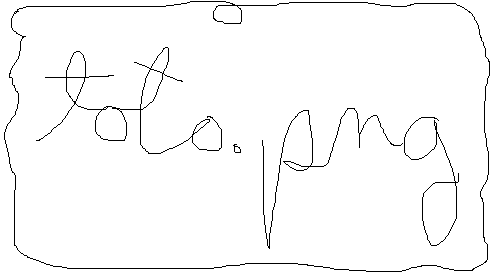
\includegraphics[width=0.97\textwidth]{toto.png}
      \caption{On peut avoir une figure sur deux colonnes.}
      \label{MaFigureDouble}
\end{figure*}



\section{Discussion et Conclusion}

C'est fini!

\addtolength{\textheight}{-12cm}   % This command serves to balance the column lengths
                                  % on the last page of the document manually. It shortens
                                  % the textheight of the last page by a suitable amount.
                                  % This command does not take effect until the next page
                                  % so it should come on the page before the last. Make
                                  % sure that you do not shorten the textheight too much.


%%%%%%%%%%%%%%%%%%%%%%%%%%%%%%%%%%%%%%%%%%%%%%%%%%%%%%%%%%%%%%%%%%%%%%%%%%%%%%%%


\begin{thebibliography}{99}
\bibitem{c1} G. O. Young, Synthetic structure of industrial plastics (Book style with paper title and editor), 	in Plastics, 2nd ed. vol. 3, J. Peters, Ed.  New York: McGraw-Hill, 1964, pp. 15-64.
\bibitem{c2} W.-K. Chen, Linear Networks and Systems (Book style).	Belmont, CA: Wadsworth, 1993, pp. 123-135.
\bibitem{c3} H. Poor, An Introduction to Signal Detection and Estimation.   New York: Springer-Verlag, 1985, ch. 4.
\end{thebibliography}

\end{document}
